\documentclass{llncs}

\usepackage{amsmath}
\usepackage{graphicx}
\usepackage{algorithmicx}
\usepackage{algpseudocode}
\usepackage{wrapfig}
\usepackage{url}

\urldef{\mailsa}\path|scj7t4@mst.edu, ff@mst.edu|

\begin{document}


\title{The Effects of Network Link Unreliability For Leader Election Algorithm in a Smart Grid System}
\author{Stephen Jackson and Bruce M. McMillin}
\institute{Computer Science Department, Missouri University of Science and Technology,
Rolla, MO 65409, USA, \email{scj7t4@mst.edu}, \email{ff@mst.edu}
}

\maketitle

\begin{abstract}
Cyber-physical systems (CPS) can improve the reliability of our critical infrastructure systems. By augmenting physical distribution systems with digital control through computation and communication, one can improve the overall reliability of a network. However, a system designer must consider what effects system unreliability in the cyber-domain can have on the physical distribution system. In this work, we examine the consequences of network unreliability on a core part of a Distributed Grid Intelligence (DGI) for the FREEDM (Future Renewable Electric Energy Delivery and Management) Project. To do this, we apply different rates of packet loss in specific configurations to the communication stack of the software and observe the behavior of a critical component (Group Management) under those conditions. These components will allow us to identify the amount of time spent in a group, working, as a function of the network reliability.
\keywords{cyber-physical systems, critical infrastructure, reliability, leader election, stability}
\end{abstract}

\section{Introduction}

Historically, leader elections have had limited applications in critical systems. However, in the smart grid domain, there is a great opportunity to apply leader election algorithms in a directly beneficial way. \cite{LOADBALANCING} presented a simple scheme for performing power distribution and stabilization that relies on formed groups. Algorithms like Zhang, et. al's Incremental Consensus Algorithm \cite{INCREMENTALCONSENSUS}, begin with the assumption that there is a group of nodes who coordinate to distribute power. In a system where 100\% up time is not guaranteed, leader elections are a promising method of establishing these groups.
A strong cyber-physical system should be able to survive and adapt to network outages in both the physical and cyber domains. When one of these outages occurs, the physical or cyber components must take corrective action to allow the rest of the network to continue operating normally. Additionally, other nodes may need to react to the state change of the failed node. In the realm of computing, algorithms for managing and detecting when other nodes have failed is a common distributed systems problem known as leader election.

This work observes the effects of network unreliability on the the group management module of the Distributed Grid Intelligence (DGI) used by the FREEDM smart-grid project. This system uses a broker system architecture to coordinate several software modules that form a control system for a smart power grid. These modules include: group management, which handles coordinating nodes via leader election; state collection, a module which
captures a global system state; and load balancing which uses the captured global state to bring the system to a stable state.

It is important for the designer of a cyber-physical system to consider what effects the cyber components will have on the overall system. Failures in the cyber domain can lead to critical instabilities which bring down the entire system if not handled properly.  In fact, there is a major shortage of work within the realm of the effects cyber outages have on CPSs \cite{CYBERRESEARCHCALL} \cite{SMARTGRIDBENEFITS}.
In this paper we present a slice of what sort of analysis can be performed on a distributed cyber control by subjecting the system to packet loss. The analysis focuses on quantifiable changes in the amount of time a node of the system could spend participating in energy management with other nodes.

\section{Background Theory}
\subsection{FREEDM DGI}
The FREEDM DGI is a smart grid operating system that organizes and coordinates power electronics and negotiates contracts to deliver power to devices and regions that cannot effectively facilitate their own need.

To accomplish this, the DGI software consists of a central component, the broker, which is responsible for presenting a communication interface and furnishing any common functionality needed by any algorithms used by the system. These algorithms are grouped into modules.

This work uses a version of the FREEDM DGI software with only one module: group management. Group management implements a leader election algorithm to discover which nodes are reachable in the cyber domain.

\subsection{Broker Architecture}

The DGI software is designed around the broker architecture specification. Each core functionality of the system is implemented within a self contained module which is provided access to core interfaces which deliver functionality such as scheduling requests, message passing, and a framework to manipulate physical devices, including those which exist only in simulation environments such as PSCAD\cite{PSCAD} and RSCAD\cite{RSCAD}.

The Broker provides a common message passing interface which all modules are allowed access to. This interface also provides the inter-module communication which delivers messages between software modules, effectively decoupling them outside of the requirement for them to be able to recognize messages addressed to them from other modules.

Several of the distributed algorithms used in the software require the use of ordered communication channels. To achieve this, FREEDM provides a reliable ordered communication protocol (The sequenced reliable connection or SRC) to the modules, as well as a ``best effort'' protocol (The sequenced unreliable connection or SUC) which is also FIFO (first in, first out), but provides limited delivery guarantees.

We elected to design and implement our own simple message delivery schemes in order to avoid complexities introduced by using TCP in our system. During development, we noticed that constructing a TCP connection to a node that had failed or was unreachable took a considerable amount of time. We elected to use UDP packets which do not have those issues, since the protocol is connectionless. From there, we were able to implement and develop our lightweight protocols which are very best effort oriented to deliver messages as quickly as possible within the following requirements.

\subsubsection{Sequenced Reliable Connection.}

The sequenced reliable connection is a modified send and wait protocol with the ability to stop resending messages and move on to the next one in the queue if the message delivery time is too long. When designing this scheme we wanted to achieve several criteria:

\begin{itemize}
\item Messages must be accepted in order - Some distributed algorithm rely on the assumption that the underlying message channel is FIFO.
\item Messages can become irrelevant - Some messages may only have a short period in which they are worth sending. Outside of that time period, they should be considered inconsequential and should be skipped. To achieve this, we have added message expiration times. After a certain amount of time has passed, the sender will no longer attempt to write that message to the channel. Instead, he will proceed to the next unexpired message and attach a ``kill'' value to the message being sent, with the number of the last message the sender knows the receiver accepted.
\item As much effort as possible should be applied to deliver a message while it is still relevant.
\end{itemize}

There one adjustable parameter, the resend time, which controls how often the system would attempt to deliver a message it hadn't yet received an acknowledgment for.

\subsubsection{Sequenced Unreliable Connection.}

The SUC protocol is simply a best effort protocol: it employs a sliding window to try to deliver messages as quickly as possible. A window size is decided, and then at any given time, the sender can have up to that many messages in the channel, awaiting acknowledgment. The receiver will look for increasing sequence numbers, and disregard any message that is of a lower sequence number than is expected. The purpose of this protocol is to implement a bare minimum: messages are accepted in the order they are sent.

Like the SRC protocol, the SUC protocol's resend time can be adjusted. Additionally, the window size is also configurable, but was left unchanged for the tests presented in this work.

\subsection{Group Management Algorithm}

Our software uses a leader election algorithm, ``Invitation Election Algorithm'' written by Garcia-Molina and listed in \cite{INVITATIONELECTION}. His algorithm provides a robust election procedure which allows for transient partitions. Transient partitions are formed when a faulty link between two or more clusters of DGIs causes the groups to temporarily divide. These transient  partitions merge when the link is more reliable. The election algorithm allows for failures that disconnect two distinct sub-networks. These sub networks are fully connected, but connectivity between the two sub-networks is limited by an unreliable link.  We have included the timeout we have set (the names are taken directly from \cite{INVITATIONELECTION}) in our tests in Table \ref{Table:Timeouts}.


%\begin{wraptable}{l}{0.5\textwidth}
\begin{table}
% increase table row spacing, adjust to taste
\caption{Group Management Timeouts}
\label{Table:Timeouts}
\centering
% Some packages, such as MDW tools, offer better commands for making tables
% than the plain LaTeX2e tabular which is used here.
\begin{tabular}{ c c }
\hline
Timeout & Duration \\ \hline \hline
Proportional Timeout & 10 - 30 seconds \\ \hline
Ready Timeout & 10 seconds \\ \hline
Invite Timeout & 5 seconds \\ \hline
Check Timeout & 15 seconds \\ \hline
Timeout Timeout & 10 seconds \\ \hline
\end{tabular}
%\end{wraptable}
\end{table}

% Check Timeout 10
% Timeout Timeout 10
% Global Timeout 5

The elected leader is responsible for making work assignments and identifying and merging with other coordinators when they are found, as well as maintaining a up-to-date list of peers for the members of his group.  Likewise, members of the group can detect the failure of the group leader by periodically checking if the group leader is still alive by sending a message. If the leader fails to respond, the querying node will enter a recovery state and operate alone until they can identify another coordinator to join with.
\subsection{Network Simulation}

Network unreliability is simulated by dropping datagrams from specific sources on the receiver side. Each receiver was given an XML file describing the  prescribed reliability of messages arriving from a specific source. The network settings were loaded at run time and could be polled if necessary for changes in the link reliability.

On receipt of a message, the broker's communication layer examine the source and select randomly based on the reliability prescribed in the XML file whether or not to drop a message. A dropped message was not delivered to any of the sub-modules and was not acknowledged by the receiver. Using this method we were able to emulate a lossy network link but not one with message delays.

\subsection{System Implementation}

The FREEDM DGI software uses a Broker Architectural pattern. This design is realized in C++ using the Boost Library\cite{BOOST}. We have also make use of other languages such as Python to provide bootstrapping and start-up routines for the software.

\subsection{How the Network Reliability Simulator Fits Into the Communication Stack}

Because the DGI's network communication is implemented using UDP, there is a listener class which is responsible for accepting all incoming messages on the socket the system is listening on. This component is responsible for querying the appropriate protocol's class to determine
if a message should be accepted. To do this, when a message is received, the message is parsed by the listener. At this point the network simulation will halt processing the  message if it should be discarded based on the defined random chance in the configuration file. Otherwise, it is delivered to the addressed module.

\section{Experimental Design}

Tests were the system were completed by applying network settings and then running the nodes in the prescribed configuration for ten minutes (using the UNIX timeout command). At this point the test was terminated and the group management system appends statistics to an output file. New settings were applied and the next test was begun.

\subsection{Tools Used, Systems Used}

The application of settings and the initiation of tests was completed using a custom script written in Python. This script used a library, Fabric \cite{FABRIC}, to start runs of the system by the secure shell (SSH). This was run on one of the machine and monitored the I/O of all nodes to ensure everything was behaving correctly.

Our experimental software also provided for ``bussing,'' where a group of edges would
have the same reliability and were iterated together, and ``fixing,'' which allowed for edges that would not change reliability across any of the runs.

All tests were run on four Pentium 4 3GHz machines with 1GB of RAM and Hyper-threading. Tests were run on an ArchLinux install using a real-time kernel, however, the snapshot of the FREEDM software used to run the tests does not feature a real-time scheduler.

The testing software was responsible for initializing instances, allowing them to run and then terminate after a fixed time limit. Additionally it provided an iterative object which generated network settings which were copied to the target machines before each test began.

Each node recorded its own state information, which was appended to a log file at termination of the run. This data was then coupled with the experimental procedure data to create the tables and charts in the results.

For each run of the system, the first 60 seconds of the system were not logged to filter out transients. This leads to a maximum recordable in-group time of nine minutes.
\subsection{Tests Performed}

Our experiments considered two configurations of the system which can be considered highly characteristic of most other scenarios. The first, a two node configuration was intended to observe a slice of the behavior of the system when two nodes (a leader and a group member) struggle to communicate with one another.

The second configuration was a four node configuration with a transient partition, where the nodes were divided into pairs. Each pair of nodes could reliably communicate with each other, but reliable communication across pairs was not guaranteed. We would vary the reliability of the connection between the pairs and observe the effects on the system.

For both tests, we ran the system using both our sequenced reliable protocol as well as our sequenced unreliable protocol. Additionally, we varied the amount of time between resends for both protocols. A full list of the tests we performed are listed in Table \ref{TableTests}.

In each test, we recorded the number of elections which began, the number that completed successfully, the amount of time spent working on elections, the amount of time spent in a group, and the mean group size. Using these metrics, we hoped to capture a good representation of what kind effects network problems could have on the stability of the groups formed.

\begin{table}[!t]
% increase table row spacing, adjust to taste
\renewcommand{\arraystretch}{1.3}
\caption{Tests Performed}
\label{TableTests}
\centering
% Some packages, such as MDW tools, offer better commands for making tables
% than the plain LaTeX2e tabular which is used here.
\begin{tabular}{c c c c c}
\hline
Test No. & Test Type & Protocol & Resend Time & Window Size \\ \hline \hline
1        & 2 Node    & SRC      & 200ms       & N/A \\ \hline
2        & 2 Node    & SUC      & 200ms       & 8 \\ \hline
3        & 2 Node    & SRC      & 100ms       & N/A \\ \hline
4        & 2 Node    & SUC      & 100ms       & 8 \\ \hline
5        & Transient & SRC      & 200ms       & N/A \\ \hline
6        & Transient & SUC      & 200ms       & 8 \\ \hline
7        & Transient & SRC      & 100ms       & N/A \\ \hline
8       & Transient & SUC      & 100ms       & 8 \\ \hline
\end{tabular}
\end{table}

\section{Results}

All results are the average of the statistics captured by each node participating, and have been grouped similarity.

\subsection{Tests 1 and 2}
Test one featured the sequenced reliable (SRC) protocol in a two node configuration with a 200ms resend time, and another run with the
the unreliable protocol (SUC) with a window size of 8. The system was configured with two DGI nodes with a transient link between them.
The mean group size is presented in Figure \ref{fig:MGS-2NODE-200}, and the amount of time in group is shown in Figure \ref{fig:IGT-2NODE-200}.

\begin{figure}[!h]
\centering
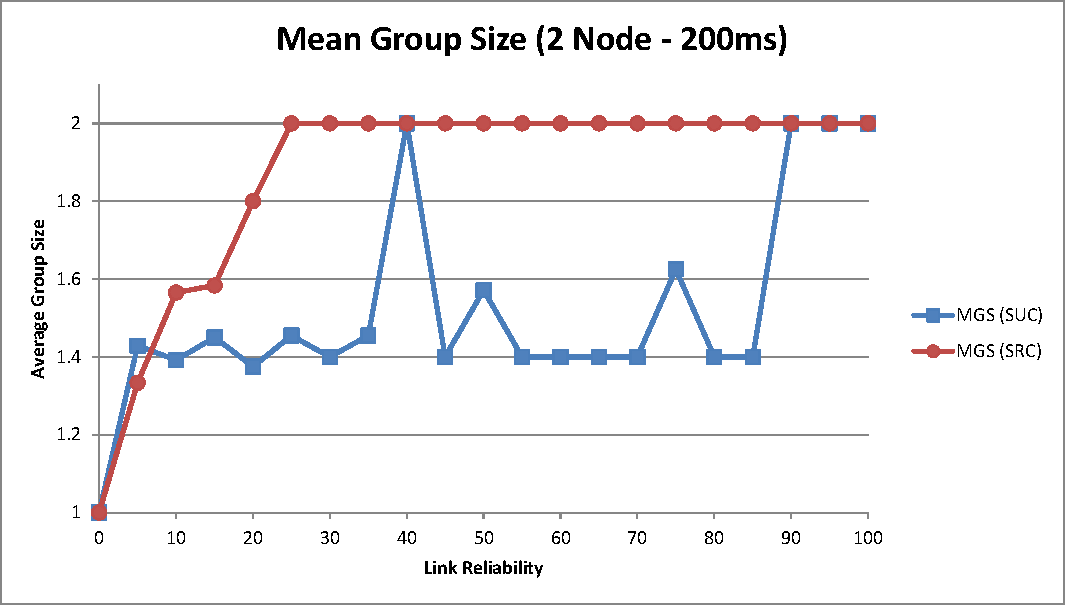
\includegraphics[width=.74\textwidth]{MGS-2NODE-200.pdf}
\caption{Average size of formed groups for two node system with 200ms resend time}
\label{fig:MGS-2NODE-200}
\end{figure}

\begin{figure}[!h]
\centering
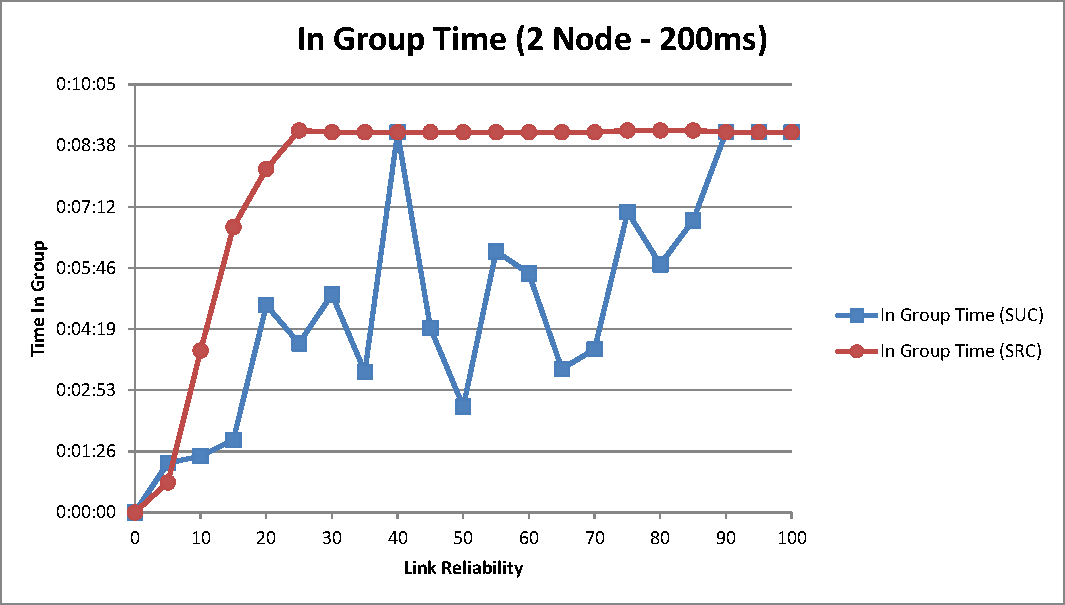
\includegraphics[width=.74\textwidth]{IGT-2NODE-200.pdf}
\caption{Total time spent in group of at least size two for two node system with 200ms resend time}
\label{fig:IGT-2NODE-200}
\end{figure}

\subsection{Test 3 and 4}

Tests 3 and 4 follow the same experimental setup as tests one and two, but the resend time has been reduced to 100ms.
The mean group size is presented in Figure \ref{fig:MGS-2NODE-100}, and the amount of time in group is shown in Figure \ref{fig:IGT-2NODE-100}.

\begin{figure}[!h]
\centering
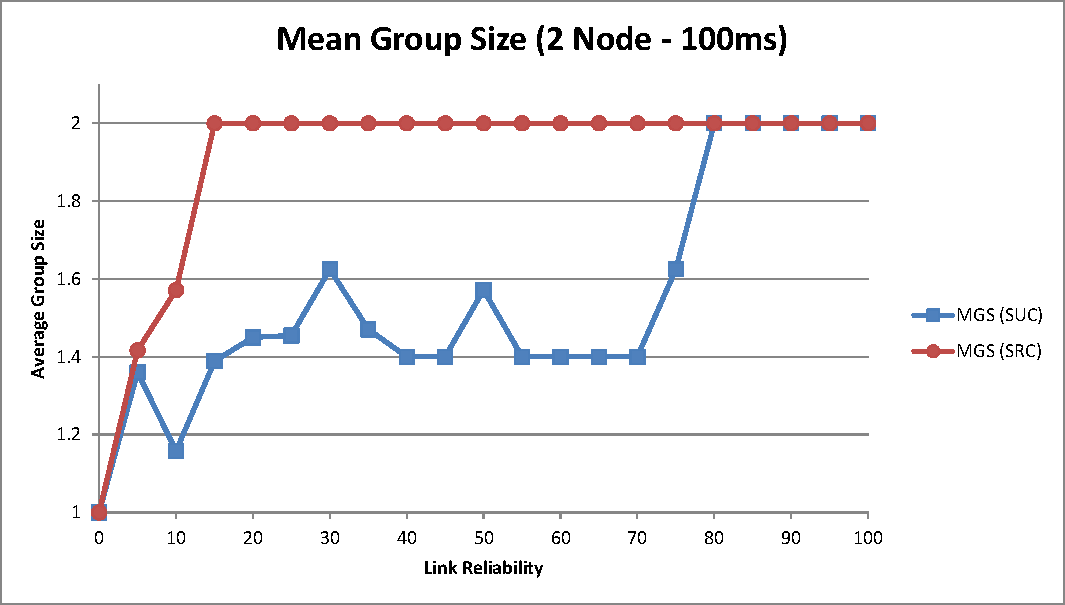
\includegraphics[width=.74\textwidth]{MGS-2NODE-100.pdf}
\caption{Average size of formed groups for two node system with 100ms resend time}
\label{fig:MGS-2NODE-100}
\end{figure}

\begin{figure}[!h]
\centering
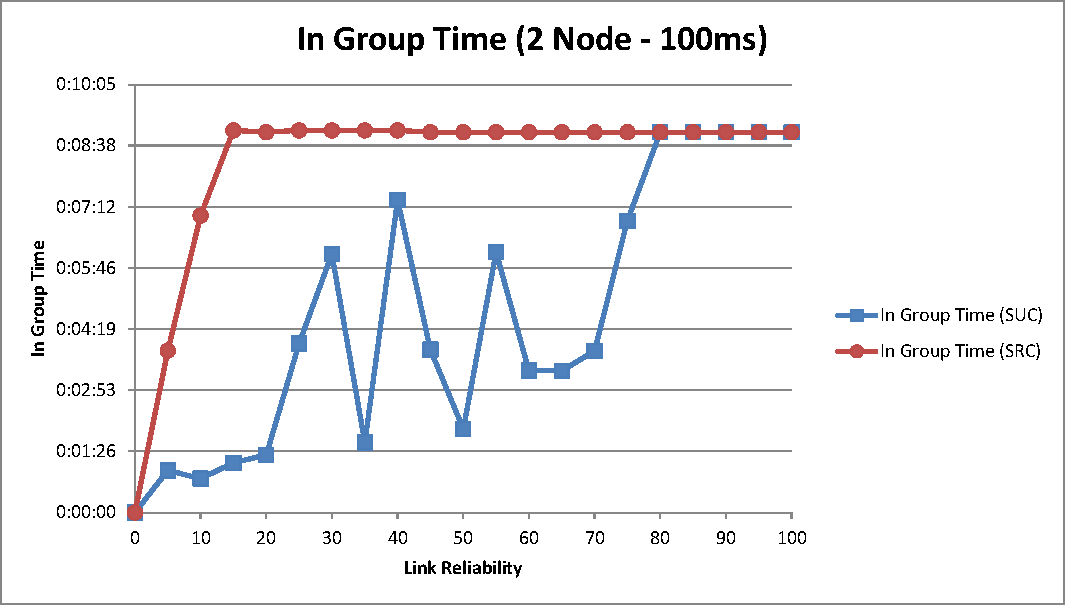
\includegraphics[width=.74\textwidth]{IGT-2NODE-100.pdf}
\caption{Total time spent in group of at least size two for two node system with 100ms resend time}
\label{fig:IGT-2NODE-100}
\end{figure}

\subsection{Test 5 and 6}

Tests five and six are the first to use the transient partition setup. The system is setup with four nodes. Two pairs of nodes are selected. Each pair of nodes can communicate without issue to each other. However, the reliability of the link between the two pairs was varied for each step of the test. These tests used a 200ms resend time. Both SRC and SUC protocols are shown here. As in the previous tests, the window size remained at 8 for the SUC protocol.

\begin{figure}[!h]
\centering
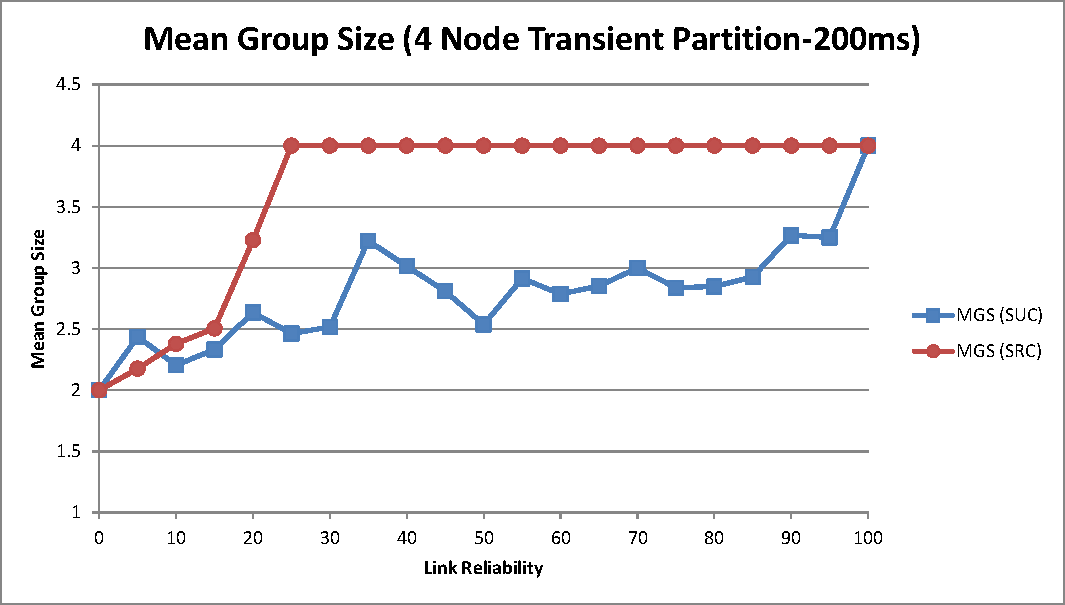
\includegraphics[width=.74\textwidth]{MGS-TRANS-200.pdf}
\caption{Average size of formed groups for a four node system with a transient partition and 200ms resend time}
\label{fig:MGS-TRANS-200}
\end{figure}

\begin{figure}[!h]
\centering
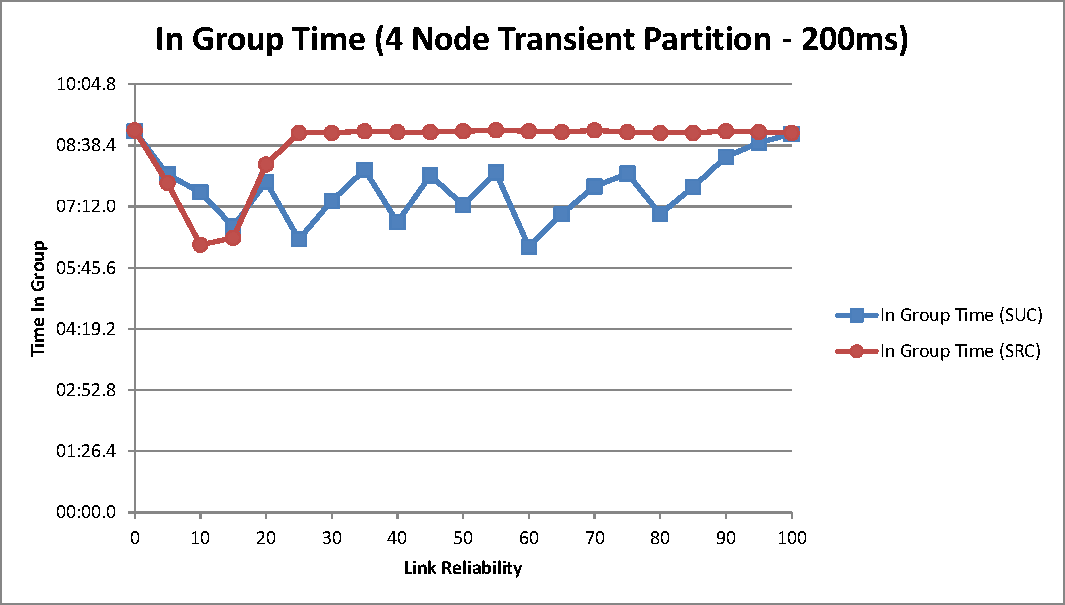
\includegraphics[width=.74\textwidth]{IGT-TRANS-200.pdf}
\caption{Total time spent in group of at least size two for a four node system with a transient partition and 200ms resend time}
\label{fig:IGT-TRANS-200}
\end{figure}

\subsection{Tests 7 and 8}

Tests seven and eight were run with the same setup as Tests 5 and 6, however the resend time was reduced to 100ms.

\begin{figure}[!h]
\centering
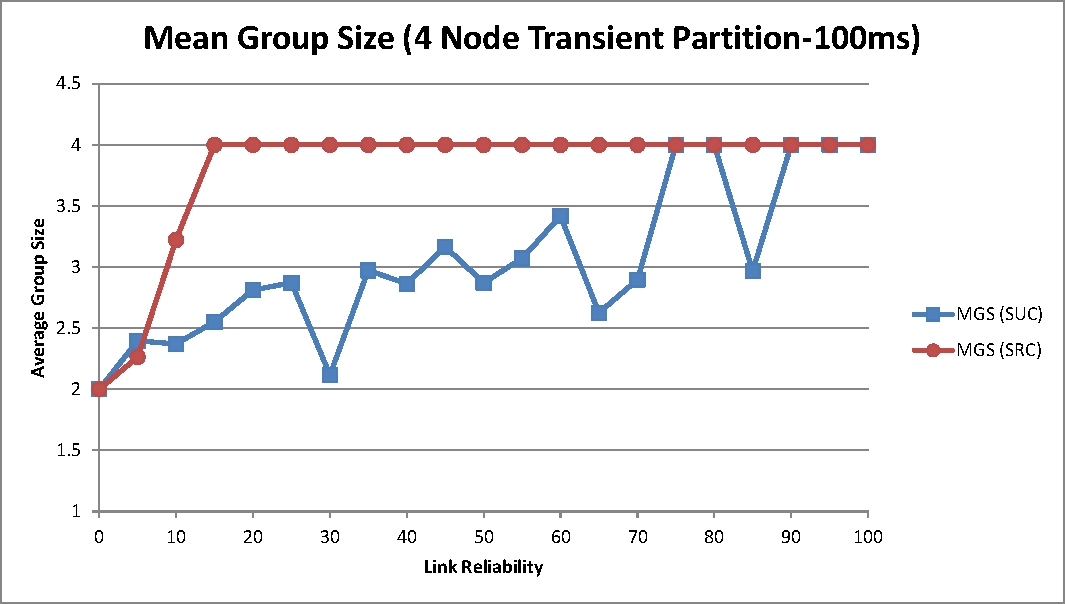
\includegraphics[width=.74\textwidth]{MGS-TRANS-100.pdf}
\caption{Average size of formed groups for a four node system with a transient partition and 100ms resend time}
\label{fig:MGS-TRANS-100}
\end{figure}

\begin{figure}[!h]
\centering
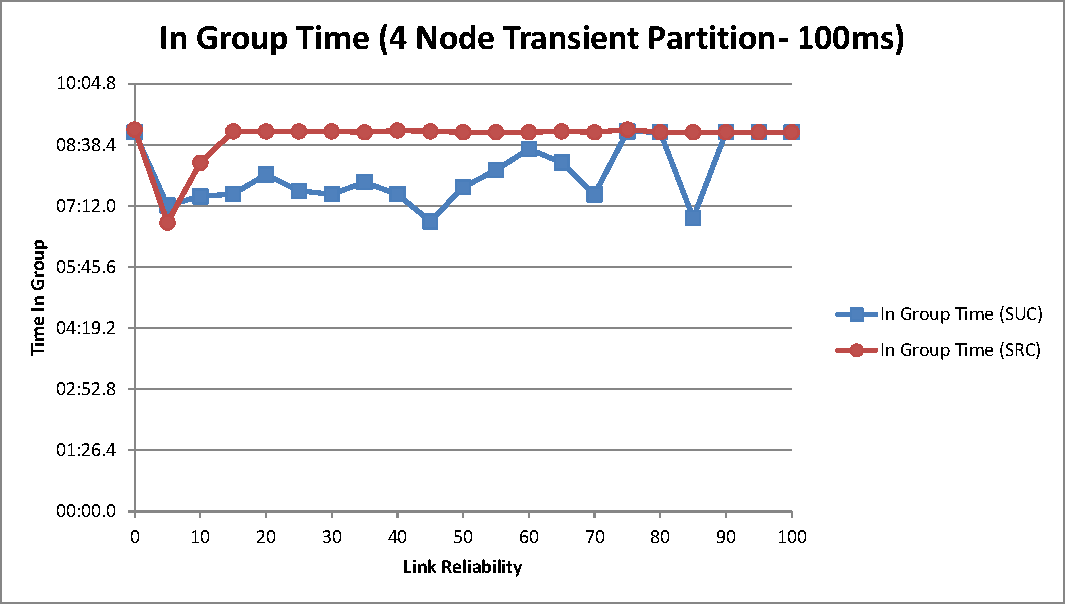
\includegraphics[width=.74\textwidth]{IGT-TRANS-100.pdf}
\caption{Total time spent in group of at least size two for a four node system with a transient partition and 100ms resend time}
\label{fig:IGT-TRANS-100}
\end{figure}

\section{Observations}

As one would expect the mean group size increases  with the stability of the link. This observation can be directly made from the data we collected. However, our measurements often included outliers such as the major one observed in Figure \ref{fig:IGT-TRANS-200}.  To confirm these points as outliers we re-ran the case (Reliability 40 with Test 2, shown in Figures \ref{fig:MGS-2NODE-200} and \ref{fig:IGT-2NODE-200}) multiple times and collected the same measurements. We collected these into Figure \ref{fig:rerun}.

\begin{figure}[!h]
\centering
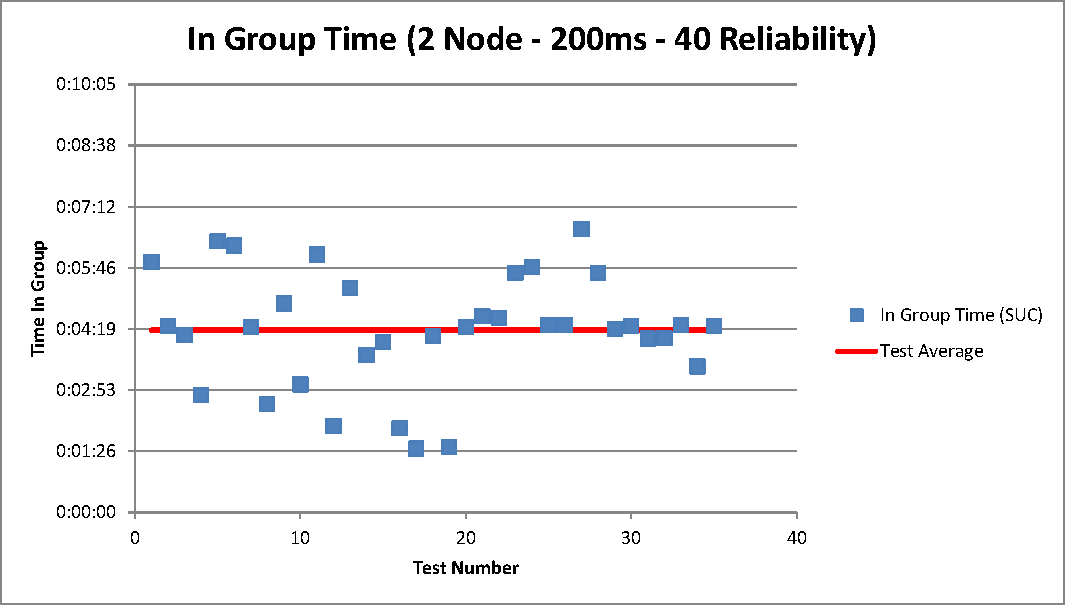
\includegraphics[width=.74\textwidth]{2NODE40RELIABILITY.pdf}
\caption{Total time spent in group of at least size two for the two node node system with the SUC protocol, 200ms resend, and 40 reliability. The average of all points is the solid line}
\label{fig:rerun}
\end{figure}

The points in Figure \ref{fig:rerun} are centered around 4m18s which is where the expected value should be based on the approximate trend of those tests.  Based on further examination, we believe points like these (since they tend to only occur with the SUC protocol) to be cause by two factors. The first factor is that SUC will ignore packets that don't arrive in increasing order, which makes situations where many messages are being passed (such as the election) more difficult to complete. The second factor is the relative stability of the formed group. The timeout for a leader or a member detecting that the other is unreachable is fairly long and given there is a relatively low amount of traffic when it is being delivered,  it is much more likely to arrive and keep the formed group alive. The outlier in Figures \ref{fig:MGS-2NODE-200} and \ref{fig:IGT-2NODE-200} is simply a case where a group formed, and the relative ease of sustaining a group kept it alive for the duration of the test. Other cases can explained similarly.

We had originally selected these two protocols to evaluate their potential in our software. As our development continued we used the SRC protocol as the default (although it is simple to switch between them). The advantages of this are obvious. As presented in nearly every test, even with fairly low link reliability very stable groups formed.  However, it does have limitations: send and wait can be slow. Although it was not relevant in these tests, with a sufficient number of messages in the system, the protocol is not capable of delivering messages fast enough to empty its waiting message queue, even with full reliability.

One of our most noteworthy observations can be made based on our transient partition cases. When the partition completely separates the two nodes, the in group time is at its maximum value.  As the reliability increases however, the transient partition causes the in group time to decrease, since the two sides of the partition are attempting to form groups with each other. This raises questions as to what happens to the underlying physical system when this happens.
\cite{NETWORKTOPOLOGY} showed that sometimes the ideal cyber network does not mimic the physical network. Then however, we have to wonder what happens when the cyber network has link failures or lost messages? Are there circumstances where a group is coordinating using a bus shared with nodes that are not in the same group allows for interactions that destabilize the system?

In the circumstances where the transient link causes an overall decrease in in group time, groups of many different sizes can form. In our case alone, groups of anywhere from one to four members can exist. In a system where coordination is made based on flow contracts \cite{LOADBALANCING}, what issues can arrive when a contract is formed with a node who leaves the group shortly thereafter? Will the effect compound if there are also physical link failures in the system?

\section{Conclusion}

In this work we have examined an application of leader election algorithms in a cyber-physical system. We showed that while there are definite benefits and uses for leader election algorithms in cyber-physical systems, they generate a flurry of new problems for system designers to deal with. We have shown that network instability can cause disruptions to the amount of service the cyber system can provide. In our analysis we questioned what the effect of transient partitions and link failures would be on the physical system, especially when the two networks are isomorphic. Our work shows that with the selection of an appropriate protocol under certain failure models, a good quality of service can be achieved in general. The transient partition case, by contrast, creates problems with group stability and is an issue to be investigated further with respect to its effect on CPSs.

\subsubsection*{Acknowledgements.} The authors acknowledge the support of the Future Renewable
Electric Energy Delivery and Management Center,
a National Science Foundation supported Engineering Research
Center under grant NSF EEC-081212, and the United States Department of Education GAANN program.

\bibliographystyle{splncs_srt}
\bibliography{report}

\end{document}


